\documentclass[l4proj.tex]{subfiles}
\begin{document}    

This chapter covers the implementation of RViT. 

\section{Software Engineering techniques}
Throughout the duration of the project, an agile approach was taken to the development of the product. The scrum framework was followed, with development being broken down into sprints, and elements of kanban framework also introduced, such as prioritising work with a kanban board.


\subsection{GitHub Version control and Continuous Integration}
GitHub was used for version control throughout the duration of the project. This ensured that back up versions of the code were available at all times, which was useful when unrecoverable local development issues occurred. As there was only one developer working on the project, no branching strategies were used, though special care was taken to write meaningful commit messages with links to the relevant user stories, so that the commit history could be accessed with ease. 

Two GitHub action workflows were used to carry out continuous integration checks on both the Django and React JS code. Both of these workflows installed the relevant dependencies, then ran a set of testing suites on the code. The Django workflow was developed roughly a month into the project, when the unit tests were first created. However, the React JS workflow was defined much later in the project, as testing did not begin until the majority of frontend code had been written. Unfortunately, due to the brittle nature of the unit tests, the continuous integration pipelines would often fail when large areas of code were refactored, so these would be disabled until time was allocated for fixing the tests. This was often not a priority, as the main way code correctness was checked was through manual testing of the application.

\subsection{Project management}
GitHub's built-in issue and project functionality were the primary tools used for the project management of RViT. The functional requirements defined in \textbf{Section 3.2} were broken down into small user stories that aligned with the INVEST criteria (\cite{Buglione2013}). This ensured that the majority of the user stories created during the development process were independent and small in scope, negotiable and valuable to the project, as well as able to be estimated and tested. 

For each user story, a definition of done was also specified to create a list of criteria, which when completed meant that the user story was done (\cite{Silva2017}). This was extremely helpful during the development process, as often user stories were defined at the start of the sprint. Therefore, having a checklist of done criteria clarified any of the ambiguous areas of a user story. Some user stories also included notes for suggested approaches to development or important development restrictions. GitHub's labels functionality was also used to categorise user stories by the development work they would require, for example, backend, frontend or testing. 

To visualise story progress and priority, a GitHub project kanban board was created and linked to RViT's repository as can be seen in \textbf{Fig. \ref{fig:My Github issue board}}. Four columns were defined to manage the workflow: 'Parking Lot', 'Backlog', 'In Progress' and 'Done'. The 'Parking lot' column was used to store issues that did not yet have user stories of definitions of done defined. These undefined issues were typically created during supervisor meetings, where scope creep occurred, or during the development process when it was realised that a story did not match the INVEST criteria, and so was broken down into more manageable pieces of work. While these stories were marked with an 'undefined' label, the labels did not show up on the project board, so an additional column was created. This visual separation helped maintain awareness of the undefined issues, and user stories and their corresponding definition of done were defined in a timely manner.

\begin{figure}[h!]
\begin{center}
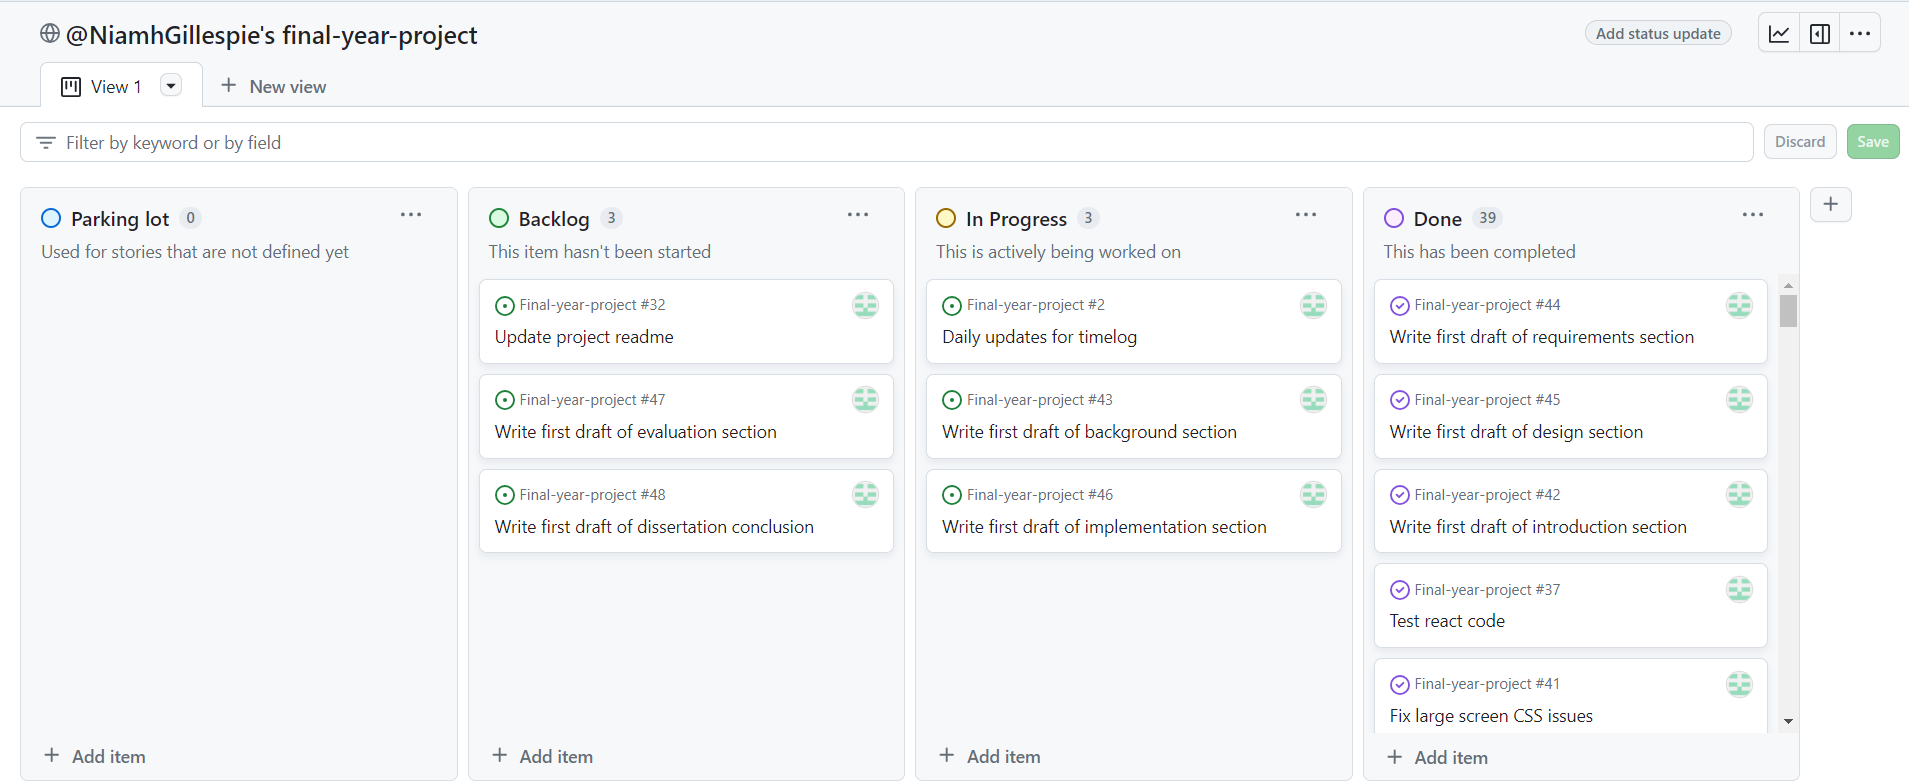
\includegraphics[scale=0.4]{dissertation/images/ImplementationIssueBoard.png}
\caption{GitHub project board used for issue management and prioritisation}
\label{fig:My Github issue board} 
\end{center}
\end{figure}


The use of a kanban board throughout project development was essential for effective management. The priority of a story in the 'Backlog' column was determined by its position with the higher-up stories having higher priority. This meant that once a story was finished, the next story to start on was easily identified. The visualisation of stories also helped with keeping track of stories that had blockers, for example, the definition of done on the majority of design tasks involved getting supervisor approval, so having these remain in the 'In Progress' column acted as a was reminder to bring these up in the supervisor meetings. The kanban board also provided invaluable in supervisor meetings, as it acted as a visual demonstration of the progress that had been made, and the user stories could also be easily accessed for further explanation.


\subsection{Sprint-based Development}
In the initial stages of the project, a kanban-style continuous flow approach was taken to development. However, this led to very fragmented development as similar requirements were often not grouped together and were worked on separately. The lack of set delivery dates also led to items being worked on for longer than they realistically should have been. To rectify these issues, areas of scrum methodology were adopted, and sprints were introduced. This meant sprint backlogs had to be defined, so similar requirements were grouped together. The backlog user stories would then be added to the kanban board so workflow could be visualised. While the sprints varied in length between three to five weeks long, time estimations also had to be calculated to discover how many issues could realistically be completed in a single sprint. 

While the time estimates were generally accurate, unforeseen blockers sometimes slowed progress down. As the project progressed it was easier to identify which kind of user stories would cause these issues, so more achievable sprint backlogs could be created. 


\subsection{Refactoring}
 As an agile approach was taken throughout the project, in line with the agile manifesto (\cite{Kent2001(manifesto)}) the creation of working software was prioritised over writing extensive documentation. This meant that for the code base to be maintainable, the code had to be well written. Approximately halfway through the project it was noticed that some improvements could be made, so a large-scale refactoring process was carried out. Both the Django and React JS sections underwent this refactor, but as more code style issues were noticed in the React JS sections, this was prioritised.

 Following advice from Kerninghan and Plauger, the code base was edited to ensure the majority of code was self-documenting and that cyclic complexity, or the presence of 'bushy trees', was reduced as much as possible (\cite{Kernignhan1974}). Cyclic complexity, or 'bushy trees', are introduced when an area of code is written that involves a high number of possible execution paths. For example, nested if statements were simplified where possible. In some of the more complex code sections such as the drag and drop functionality, large areas of the code were re-written to improve code comprehension. Special care was also taken to ensure variable names were as self-documenting as possible. There was also a repeated code, particularly across the React JS classes, so as much of this code as possible was refactored into helper functions. Unfortunately, due to a majority of functions carrying out class state updates, not as many of these functions were able to be refactored. The file structure of the React JS code was also improved, with files split into various sub-folders rather than being all at one level. 

 To ensure consistent use of white space, and to make sure the code written was up to professional standard of readability, all React JS code was linted. ESLint was used to identify common JavaScript problems such as syntax errors and other code smells, while Prettier was used to provide an opinionated style guide to ensure a consistent coding style was followed throughout the JavaScript code base. This tooling was used consistently during the rest of the project to ensure good quality code was written.


\section{API Implementation}
As discussed in the design chapter, the API was developed throughout the duration of the project. This meant that the API implementation was regularly changed as new features were added. Towards the end of the project, administration support was added. This feature set implemented team and user functionality, so the majority of API endpoints had to be refactored to account for these changes. 

This was mostly a consequence of the order in which development was carried out. However, if future work was conducted where the API was used across different platforms, any changes to endpoint functionality would have to be carefully considered, to avoid introducing breaking changes if possible.

\section{Frontend}

\subsection{Components}
The use of components was essential when developing RViT. This allowed dashboards with large feature sets to be broken down into smaller, more manageable files. The components were also reusable across the code base, meaning code did not have to be redeveloped for different use cases. This also meant that if updates were needed to refine the display, or use of a component, it only needed to be edited in one file rather than in multiple places. 

Using components also allowed for updates to be carried out on these without having to refresh the entire page. This leads to quicker loading times for the user and was essential when implementing pages like the Tracking Dashboard where a user stories state can be updated without a full-page refresh needed. 

\subsection{Drag and Drop}
As the Epics Dashboard was designed to let users visualise priority by the spatial ordering of epics and user stories, users needed to be able to reorder these elements. It was decided that the most user-friendly way to implement this was through the use of drag and drop. A library was used to provide this functionality as developing these features would have taken up too much project time. 

A number of react libraries were tested, with the majority of them found to be lacking the appropriate documentation or example code for the required functionality to be properly implemented. Finally, the react-beautiful-dnd library was chosen as it had an appropriate amount of documentation and is also widely used with over 1,000,000 weekly downloads (\cite{ReactDnD}). The learning curve was still steep as RViT's elements had to have both draggable and droppable sections in order to work correctly. 

It was noticed that it could be quite difficult for a user to re-order the user stories due to the limited space they took up on the page, so colour feedback was provided to highlight where the user story could be dropped. To further customise the user experience this colouring was based on the colour of the epic that the user story corresponded to. 

While the implementation on the Epics Dashboard only allowed for the epics to be reordered horizontally and the user stories vertically, the Tracking Dashboard required both horizontal and vertical movement of the user stories between columns. While the same library was used, the implementation of the functionality was quite different. In the Epics Dashboard, each epic and user story was given an ordering number that would be updated when a drag and drop event occurred. This ensured the ordering remained consistent across all team members. However, for the Tracking Dashboard an ordered list of stories was maintained to carry out this functionality. If a story was moved out of a column, it was removed from the list, and if a story was moved into a column, it was added to the list at the appropriate position. If a story was reordered in a column, the list was updated to reflect the new positioning. While this led to more API calls being made, it was essential to making sure that every member of a team could view the boards and see the same ordering. A code snippet featuring the drag and drop from the Tracking column dashboard can be seen in \textbf{Listing \ref{listing: drag and drop}}

\begin{lstlisting}[caption= Drag and drop code snippet from the Tracking Dashboard]
if (columns !== undefined) {
    return_list.push(
        <DragDropContext
            onDragEnd={(result) => {
                if (!result.destination) {
                    return;
                }

                this.reorderStories(result.destination, result.draggableId, result.source.droppableId, result.source.index);
            }}>
            
            {columns.map((column, index) => (
                <Droppable key={column.id} droppableId {column.id.toString()}>
                    {(provided, snapshot) => (
                        <div {...provided.droppableProps} ref={provided.innerRef} className="d-flex">
                            <div
                                className="column-container"
                                droppableId={column}
                                style={getDraggingStyleColumn(snapshot.isDraggingOver, column.WIP, column.stories)}>
                                <EditColumnModal
                                    className="pb-0 mb-1"
                                    resetState={this.resetState}
                                    column={column}
                                    non_completed_stories={non_completed_stories}
                                    team={this.state.team}
                                />
                    
                                {column.WIP !== 0 ? (
                                    <p className="wip-limit mt-0 mb-2 d-block" style={WIPStyling(column.WIP, column.stories)}>
                                        WIP: {column.WIP}
                                    </p>
                                ) : (
                                    <p className="no-wip-limit mt-0 mb-2 d-block"> </p>
                                )}
                                <hr className="pt-0 mt-2 d-block w-100"></hr>

                                {this.displayStories(column)}
                                {provided.placeholder}
                            </div>
                        </div>
                    )}
                </Droppable>
            ))}
        </DragDropContext>
    );
}
\end{lstlisting}
\label{listing: drag and drop} 

\subsection{Styling}
The use of colour was essential to creating an easy-to-use approach to agile project management. Users could set the colours of epics, tags and values through the use of a colour picker as seen in \textbf{Fig. \ref{fig:Tag form colour example}}. User stories inherited their colour from the epic they belonged to, creating an easy visual connection between elements. These colours persisted throughout the application, which was achieved though inline CSS styling. 

\begin{figure}[h!]
\begin{center}
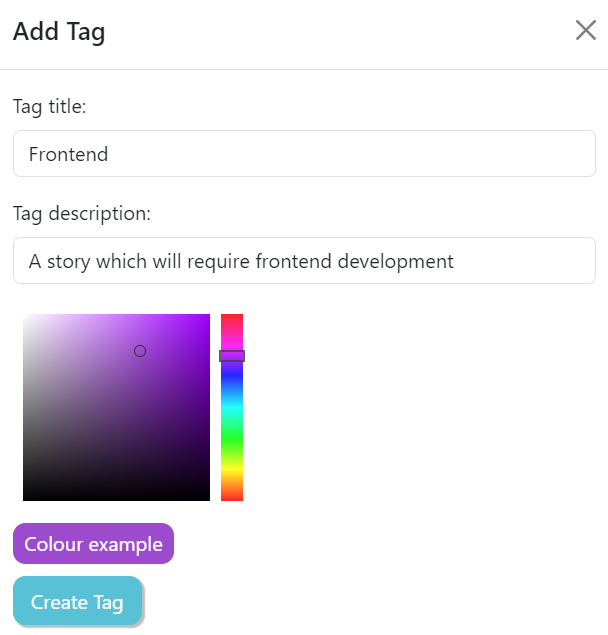
\includegraphics[scale=0.4]{dissertation/images/TagFormColourExample.png}
\caption{Add Tag form featuring the colour picker}
\label{fig:Tag form colour example} 
\end{center}
\end{figure}

The majority of styling was carried out through Bootstrap and external CSS. Bootstrap was used primarily for the easy positioning of elements, while CSS was used to style fully custom component designs that could easily be refactored. 

\section{State Management}
To ensure the consistency of state between components, state management was used. To ensure the dashboard information was up to date, on page load or refresh the relevant states were set through API calls. State was then passed through React Props to the page's relevant components to ensure the correct information was displayed. 

If any of the components were updated, the relevant POST requests would be carried out to update the database and ensure consistency across users.


\section{Help Documentation}
As more features were added to RViT, the application became more complex, so in-app help documentation was added to assist users. It was decided to keep the length of this documentation to a minimum while still explaining the key areas of the application. This was to ensure it could be read quickly by developers and that they would not be slowed down by reading any unnecessary details. 

It was also decided to localise this documentation on a separate web page instead of throughout the application. This was to avoid cluttering the user interface with help tool-tips or pop-ups that would not be needed by users experienced with the tool. The documentation was split into subsections; a general overview of what RViT is, followed by a 'how to use' section for each user type describing the different pages and functionality they will have access to.

This documentation should be expanded in the future, especially as it currently expects the user to understand key agile concepts such as what an epic is and how kanban boards work. This would not be ideal for users new to either agile overall or the kanban framework in particular. 

\section{Security}
The three-tier architecture protects RViT from the majority of scripting attacks due to the lack of direct communication between the presentation and data tiers. Vigorous form validations were carried out on the client side of the application, with users kept aware of if they had met requirements on type. To further limit the possibility of a scripting attack, all test form fields were assigned a maximum number of characters that a user could enter.

JSON web tokens (JWTs) were used for authorisation. Upon a successful log in attempt, the API generated a unique JWT to verify the user's identity, which is then sent to the web application and stored for future use. When an API request for a protected resource is sent, the JWT will be sent to the API via the header where it will be verified and if valid, the request will be completed.  

\section{Deployment}
At the end of the project, once RViT's core functionality had been completed, a deployment was planned. It was decided to host the Django API and database separately from the React JS application. This allowed the API to be hosted and tested from the locally hosted version of the RViT web application to make ensure the API worked as expected prior to the React JS application being hosted.

It was decided to use Python Anywhere to host the Django API and database. This was primarily chosen due to the author's previous experience working with the tool in addition to the free tier provided, which allocated enough CPU runtime and disk storage to successfully host the API and database. It was noticed that the locally hosted version of RViT did begin to experience some short lags once the API calls were being processed using the hosted API, but as seen in the performance evaluation, these did not affect the usability of the web application greatly.

The application tier was then hosted using Netlify. Similarly to Python Anywhere, this provided a free tier that suited the project's needs. Netlify also linked straight to RViT's GitHub repository meaning the web application could be updated each time a commit was made. This was especially helpful when fixing display issues on screens of different sizes as the code could be committed straight to RViT's repository, and Netlify would update the web application rapidly.
\end{document}
